
\documentclass[../../../all/physics-standard_questions_all.tex]{subfiles}

\graphicspath{{../../../../figures/}}

\begin{document}

\begin{enumerate}

    \item 図のように，電池E$_1$（起電力$3V_0$），E$_2$（起電力$V_0$），電気抵抗R$_1$（抵抗値$2R$），
    R$_2$（抵抗値$2R$），R$_3$（抵抗値$R$）からなる回路がある．
    AB間を流れる電流の大きさ$I$を求めよ．
    %
    \par \vspace{0.2\baselineskip}
    {\centering
        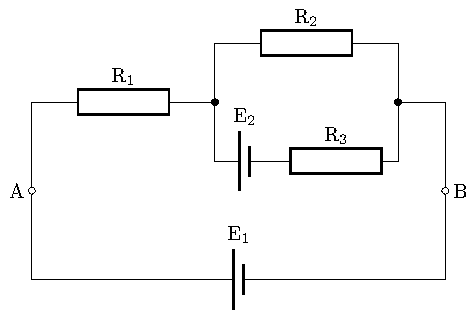
\includegraphics{q_circuit-basics_08_01/physics-standard_questions_circuit-basics_08_01_tikz.pdf}
    \par}
    \vspace{0.2\baselineskip}
    
    \item 図のように，電池E（起電力$V_0$），電気抵抗R$_1$（抵抗値$R$），R$_2$（抵抗値$R$），
    R$_3$（抵抗値$R$），R$_4$（抵抗値$3R$），R$_5$（抵抗値$R$）からなる回路がある．
    AB間を流れる電流の大きさ$I$を求めよ．
    %
    \par \vspace{0.2\baselineskip}
    {\centering
        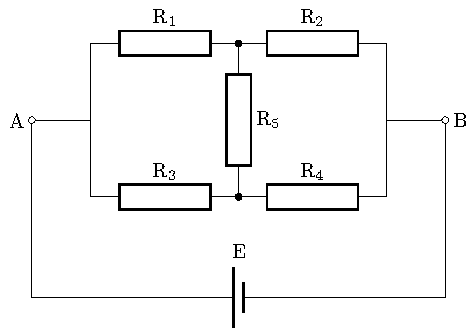
\includegraphics{q_circuit-basics_08_02/physics-standard_questions_circuit-basics_08_02_tikz.pdf}
    \par}
    \vspace{0.2\baselineskip}

\end{enumerate}

\end{document}
